\documentclass[xcolor={dvipsnames}]{beamer}
\usepackage{HECbeamer}
\uselanguage{French}
\languagepath{French}
\title[\color{white}{MATH60604 \S~2h - Colinéarité}]{MATH60604 \\Modélisation statistique \\ \S~2h - Colinéarité}
\author{}
\date{\today}
\institute{HEC Montréal\\
Département de sciences de la décision}
\date{} 

\begin{document}
\frame{\titlepage}
\section{Multicolinéarité}

\begin{frame}
\frametitle{Multicolinéarité}
\bi
\item On dit que deux covariables $\mathrm{X}_1$ et $\mathrm{X}_2$ sont \alert{colinéaires} si
\bi
\item $\mathrm{X}_1$ et $\mathrm{X}_2$ sont toutes deux corrélées avec $Y$
\item $\mathrm{X}_1$ et $\mathrm{X}_2$ sont fortement corrélées entre elles --- elles contiennent essentiellement la même information.
\ei
\item Il peut y avoir de la multicolinéarité entre plus de deux variables\ldots de la même façon qu'il pourrait y avoir plus d'un facteur confondant.
\item Dans ce cas, la \alert{multicolinéarité} (ou  colinéarité) sert à décrire le cas de figure où une (ou plusieurs) variable explicative est fortement corrélée avec une combinaison linéaire des autres covariables.
\item Une conséquence nuisible de la multicolinéarité est la \alert{perte de précision} dans l'estimation des paramètres, et donc l'augmentation des erreurs-type des paramètres. 
\ei
\end{frame}



\begin{frame}
\frametitle{Un exemple débile pour illustrer la colinéarité}
\bi
\item Considérez le log du nombre quotidien de locations de Bixi  en fonction de la température en degrés Celcius et Farenheit (et la température en ${}^{\circ}$F arrondie au degré près). Soit le modèle linéaire 
\begin{align*}
 \code{lognutilisateur} = \beta_0 + \beta_{\code{c}} \code{celcius} + \beta_{\code{f}} \code{farenheit} + \varepsilon.
\end{align*}
\item L'interprétation de $\beta_{\code{c}}$ est « le facteur d'augmentation du nombre de locations quotidiennes quand la température croît de $1{}^{\circ}$C, tout en gardant la température F constante »\ldots
\item Les deux unités de températures sont liées par la relation linéaire
\[1.8 \code{celcius} + 32= \code{farenheit}.\]
\ei
\end{frame}
\begin{frame}
\bi \item 
 Supposons que le vrai effet  (fictif) de la température sur le log du nombre de locations de vélo est
 \begin{align*}
  \code{lognutilisateur} = \alpha_0+ \alpha_1 \code{celcius} + \eps.
 \end{align*}
\item Les coefficients du modèle qui n'inclut que la température Farenheit sont donc
 \begin{align*}
  \code{lognutilisateur} = \gamma_0 + \gamma_1\code{farenheit} + \eps.
 \end{align*}
 où $\alpha_0 = \gamma_0 + 32\gamma_1$  et $1.8\gamma_1 = \alpha_1$.
 \item Les paramètres du modèle postulé avec les deux variables, 
 \begin{align*}
 \code{lognutilisateur} = \beta_0 + \beta_{\code{c}} \code{celcius} + \beta_{\code{f}} \code{farenheit} + \varepsilon,
\end{align*}
 ne sont pas \textbf{identifiables}: n'importe laquelle combinaison linéaire des deux solutions
 %Pour tout $k$, $\beta_0 = k\alpha_0 + (1-k)\gamma_0$, $\beta_{\code{c}}=k\alpha_1$ et $\beta_{\code{f}}=(1-k)\gamma_1$ 
 donne le même modèle ajusté.
\ei
\end{frame}

\begin{frame}[fragile]
 \frametitle{Bixi et multicolinéarité}
 On utilise des données tirées du site de Bixi avec la température à 16h (\code{rfarenheit} dénote la température Farenheit arrondie) pour expliquer le nombre de locations quotidiennes entre 2014 et 2019.
    \begin{figure}[ht!]
 \centering 
  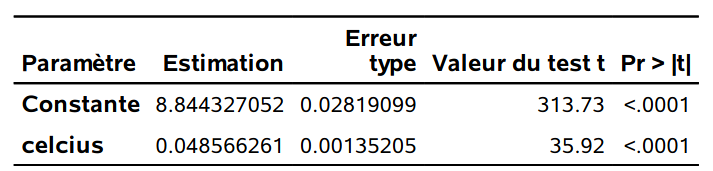
\includegraphics[width = 0.49\textwidth]{img/c2/diapos3-e20} 
  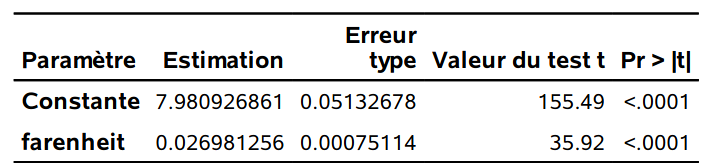
\includegraphics[width = 0.49\textwidth]{img/c2/diapos3-e21}
 \end{figure}
 
   \begin{figure}[ht!]
 \centering 
  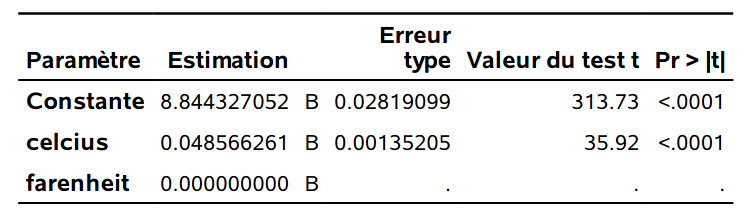
\includegraphics[width = 0.49\textwidth]{img/c2/diapos3-e22} 
  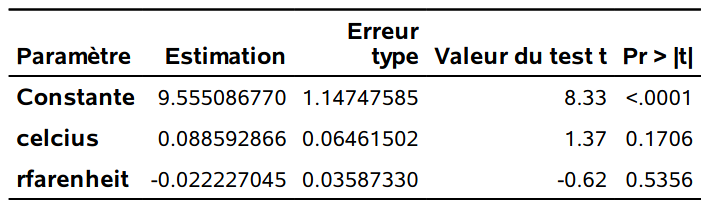
\includegraphics[width = 0.49\textwidth]{img/c2/diapos3-e23}
 \end{figure}
 {\footnotesize \SASlang imprime un avertissement en cas de colinéarité.
 \begin{quote}
 \textbf{Note}: The X'X matrix has been found to be singular, and a generalized inverse was used to solve the normal equations. Terms whose estimates are followed by the letter 'B' are not uniquely estimable.
 \end{quote}
 
 }


\end{frame}
\begin{frame}{Effet de la colinéarité}

Règle générale, la colinéarité a les impacts suivants:
\bi
\item Les estimés des coefficients changent drastiquement quand de nouvelles observations sont ajoutées au modèle, ou quand on ajoute/enlève des variables explicatives.
\item Les erreurs-type des coefficients de la régression linéaire sont très élevées, parce que les $\bs{\beta}$ ne peuvent pas être estimés précisément.
\item Conséquemment, les intervalles de confiance pour ces coefficients sont très larges.
\item Les paramètres individuels ne sont pas statistiquement significatifs, mais le test $F$ pour l'effet global du modèle indiquera que certaines variables sont utiles.
\ei

\end{frame}

\begin{frame}[fragile]
\frametitle{Comment détecter la multicolinéarité et les facteurs confondants?}
\bi
\item Si les variables sont exactement colinéaires, \SASlang et \Rlang en enlèvera une {\footnotesize (\SASlang imprime la même remarque que lorsque vous déclarez des variables catégorielles à l'aide de  \code{class})}.
\bi 
\item Les variables qui ne sont pas \textbf{parfaitement} colinéaires (par exemple arrondies) ne seront pas détectées par le logiciel et poseront problème.
\ei
\item On peut regarder la \textbf{corrélation linéaire} entre \alert{variables explicatives} et les changements dans les estimés des paramètres pour les régressions avec et sans certaines variables.
\item Quand il y a plus de deux variables multicolinéaires, la détection est moins facile.
\item Une variable explicative peut être corrélée avec une combinaison linéaire d'autres variables sans forcément avoir une corrélation très forte avec les variables individuelles. 

\ei
\end{frame}

\begin{frame}
\frametitle{Facteur d'inflation de la variance}

\bi
\item Un autre outil pour détecter la multicolinéarité est le facteur d'inflation de la variance ($\mathsf{VIF}$). 
\item Pour une variable explicative donnée $\mathrm{X}_j$, son $\mathsf{VIF}$ est
\begin{align*}
\mathsf{VIF}(j)=\frac{1}{1-R^2(j)}
\end{align*}
où $R^2(j)$ est le $R^2$ du modèle obtenu en régressant $\mathrm{X}_j$ sur les autres variables explicatives.
 \item On parle parfois de facteur de tolérance, $\mathsf{TOL}=1-R^2(j)$, soit la réciproque du $\code{VIF}$.
 \ei
 \end{frame}
 \begin{frame}
 \frametitle{Quand est-ce que la colinéarité est problématique?}
 \bi
\item $R^2(j)$ représente la proportion de la variance de $\mathrm{X}_j$ qui est expliquée par les autres prédicteurs.

\item Il n'y a pas de concensus mais, règle générale, 
\bi 
\item $\mathsf{VIF}(j) > 4$ ou $\mathsf{TOL} < 0.25$ si $R^2(j) >0.75$
\item $\mathsf{VIF}(j) > 5$ ou $\mathsf{TOL} < 0.2$ si $R^2(j) >0.8$
\item $\mathsf{VIF}(j) > 10$ ou $\mathsf{TOL} < 0.1$ si  $R^2(j) >0.9$.
\ei
\ei
\end{frame}

\begin{frame}
 \frametitle{Multicolinéarité et Bixi}
 \bi 
  \item La valeur de la statistique $F$ pour le test de significativité globale (omise de la sortie) du modèle linéaire simple avec température Celcius est $1292$ avec une valeur-$p$ de moins de $0.0001$; cela suggère que la température est un excellent prédicteur ($5$\% d'augmentation du nombre d'utilisateurs pour chaque augmentation de $1^{\circ}$C).
 \item En revanche, dès qu'on inclut Celcius et Farenheit (arrondi au degré près), les coefficients individuels ne sont plus statistiquement significatifs à niveau $5\%$. 
 \item Qui plus est, le signe du coefficient de \code{rfarenheit} est différent de celui du modèle avec \code{farenheit}!
   \item Remarquez que les erreurs-type de Celcius sont $48$ fois plus grandes dans le modèle avec les deux variables.
 \item Les facteur d'inflations de la variance  de \code{celcius} et \code{rfarenheit} sont énormes ($2282$) et permet de diagnostiquer le problème. 
\ei
\end{frame}
\begin{frame}[fragile]
 \frametitle{Diagrammes de régression partielle pour Bixi}
 
 \begin{figure}
  \centering 
  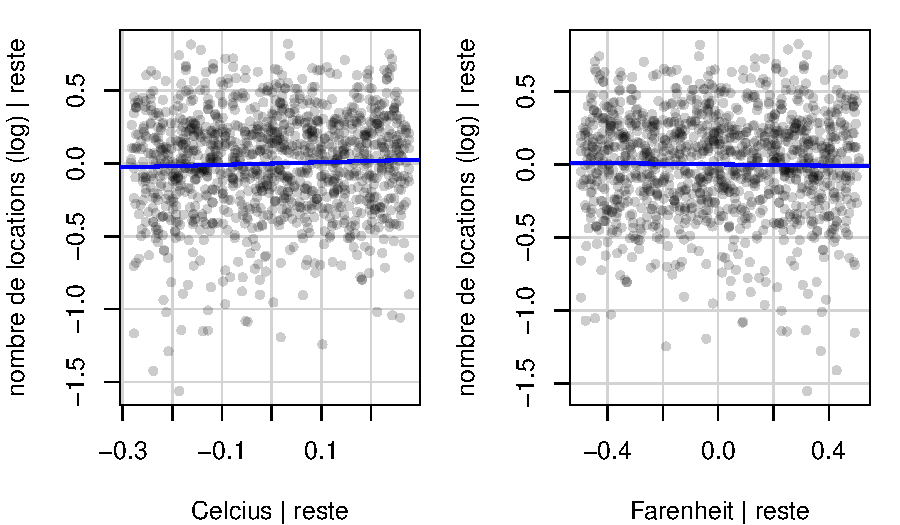
\includegraphics[width = \textwidth]{img/c2/03-linreg-avplot_temp_fr.pdf}
 \end{figure}

\end{frame}




\begin{frame}
\frametitle{Exemple fictif d'un modèle avec un problème de multicolinéarité}
\bi
\item Voici un exemple fictif avec 100 observations d'une variable réponse 
$Y$ avec cinq variables explicatives  $\mathrm{X}_1$ à $\mathrm{X}_5$
\item Les données sont dans la base de données \code{simcolineaire.sas7bdat}.
\item  En réalité, les valeurs de $Y$ ont été générées aléatoirement selon le modèle
\begin{align*}
Y=\mathrm{X}_1+\mathrm{X}_2+\mathrm{X}_3+\mathrm{X}_4+\mathrm{X}_5+\varepsilon
\end{align*}
\item Le paramètre associé à chaque variable explicative est $1$.
\ei
\end{frame}

\begin{frame}[fragile]
\frametitle{Exemple fictif de multicolinéarité}
Voici d'abord la matrice des corrélations entre toutes ces variables.
\begin{tcolorbox}[colback=white,colframe=hecblue,title=code \SASlang pour la corrélation]
\begin{verbatim}
proc corr data=infe.simcolineaire noprob;
var y x1-x5;
run;
\end{verbatim}
\end{tcolorbox}
\begin{center}
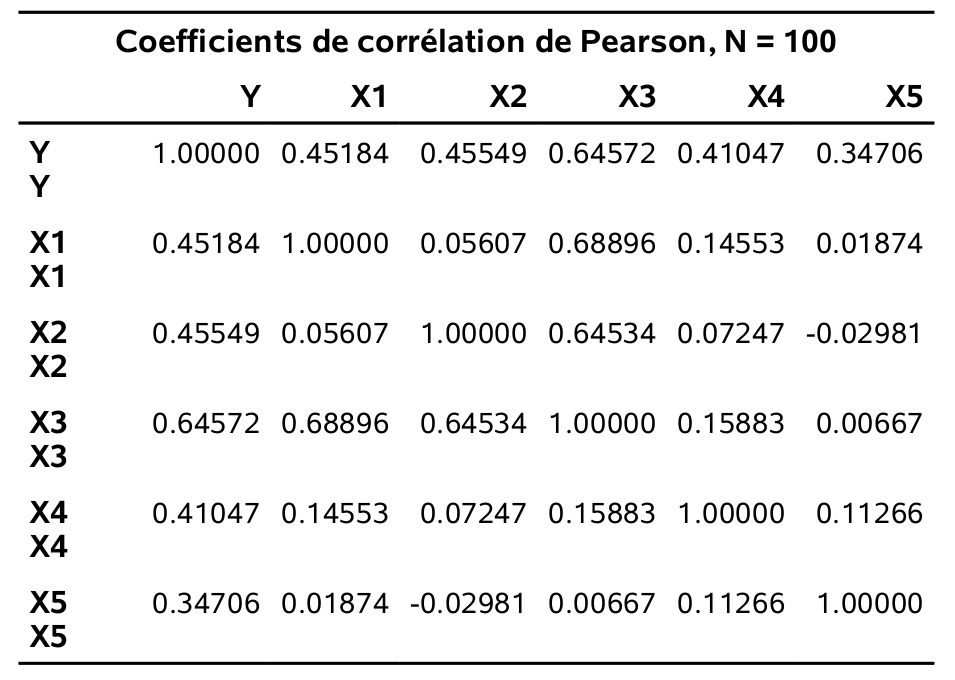
\includegraphics[width= 0.6\linewidth]{img/c2/diapos3-e24}
\end{center}

\end{frame}

\begin{frame}[fragile]
\frametitle{Modèle linéaire simple pour l'exemple fictif}
\bi
\item La corrélation entre $Y$ et chaque variable explicative est significative et
positive. 
\item Par conséquent, si on ajustait séparément les cinq modèles avec une
seule variable explicative à la fois, le paramètre de la variable serait significatif
et positif à chaque fois. Ceci est cohérent avec le vrai modèle qui a généré les
données. 
\item Ceci démontre aussi qu'il y a assez d'observations pour bien estimer
les paramètres et avoir les bonnes conclusions quant à leurs effets, du moins
lorsque qu'on les considère un à la fois.
\ei
\end{frame}

\begin{frame}[fragile]
\frametitle{Exemple fictif de multicolinéarité}
\bi
\item En revanche, $\mathrm{X}_1$, $\mathrm{X}_2$ et $\mathrm{X}_3$ sont très corrélées entre elles, ce qui peut causer un problème de multicolinéarité.
\item Ajustons d'abord le modèle contenant toutes les variables explicatives avec \code{proc reg} tout en
demandant les diagnostics de multicolinéarité.
\vp \vp
\begin{tcolorbox}[colback=white,colframe=hecblue,title=Code \SASlang pour calculer les facteurs d'inflation de la variance]
\begin{verbatim}
proc reg data=infe.simcolineaire; 
model y=x1-x5 / vif; 
run;

proc glm data=infe.simcolineaire;
model y=x1-x5 / ss3 solution tolerance;
run;
\end{verbatim}
\end{tcolorbox}
\ei
\end{frame}
\begin{frame}{Procédures \code{reg} versus \code{glm} en \SASlang}
La procédure \code{reg} permet également d'ajuster des modèles linéaires dans \SASlang.
\bi \item Par défaut, les graphiques sont imprimés (option \code{plots=diagnostics} dans \code{glm}).
\item La procédure \code{reg} a des fonctionnalités pour la sélection de modèle (pas utile en inférence).
\item Le tableau des coefficients est également imprimé (option \code{solution} dans \code{glm}).
\item En revanche, la procédure \code{reg} ne permet pas d'inclure des variables catégorielles: ces dernières doivent \textbf{obligatoirement} être encodées à l'aide de variables indicatrices binaires (\code{0}-\code{1}) (\textbf{erreur fréquente}).
\item  Dans \SASlang, on peut utiliser l'option \code{vif} dans la procédure \code{reg} ou \code{tol} (réciproque du $\mathsf{VIF}$) avec les procédures \code{reg} et \code{glm}.
\ei
 
\end{frame}


 \begin{frame}
\frametitle{Estimés des paramètres et des VIF}
\begin{center}
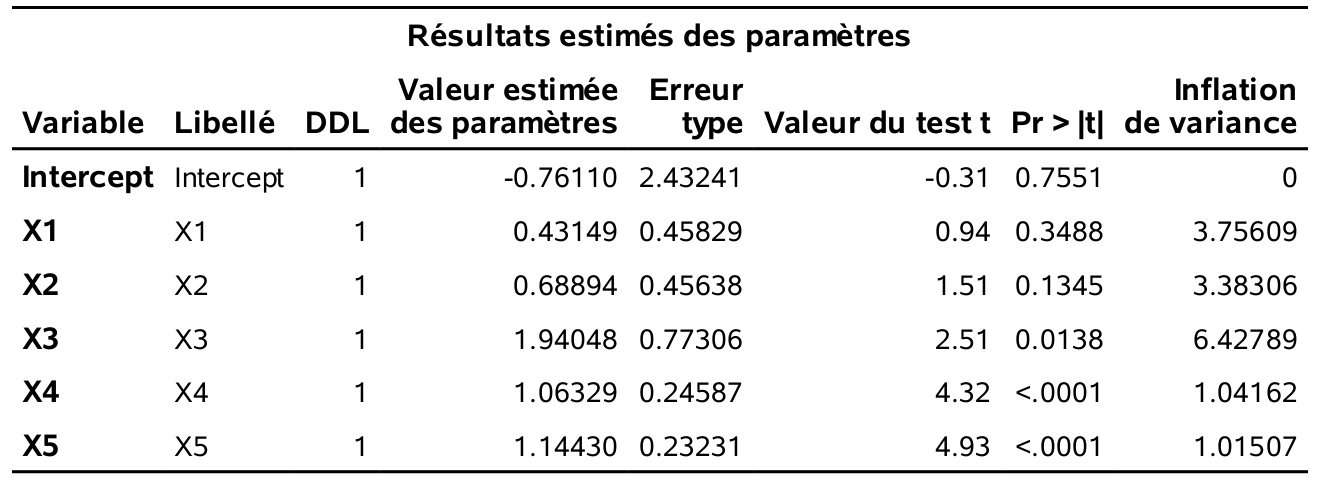
\includegraphics[width= 0.8\linewidth]{img/c2/diapos3-e25}
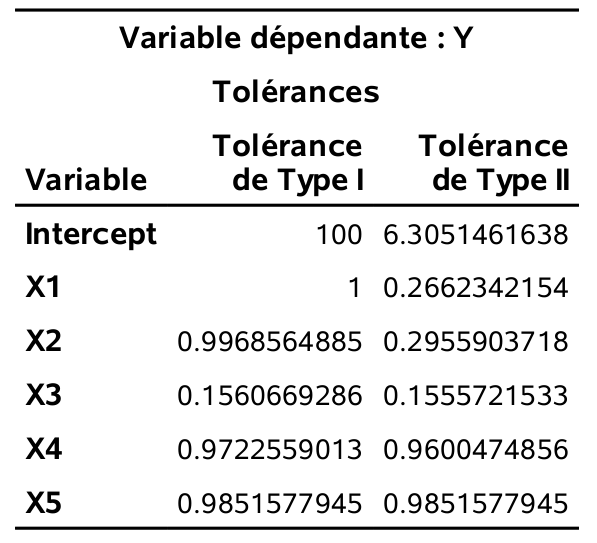
\includegraphics[width= 0.4\linewidth]{img/c2/diapos3-e26}
\end{center}
\end{frame}

\begin{frame}[fragile]
\frametitle{Adéquation pour l'exemple fictif de multicolinéarité}
\bi
\item Dans l'ensemble, le modèle semble adéquat; le  $R^2$ est de $62\%$. 
\item En revance, les coefficients $\mathrm{X}_1$ et $\mathrm{X}_2$ ne sont pas significatifs une fois les autres variables prises en compte.
\item Les facteurs d'inflation de la variance $\mathsf{VIF}$ de $\mathrm{X}_3$ est grand ($6.43$) et ceux de $\mathrm{X}_1$ et $\mathrm{X}_2$ oscillent entre $3$ et $4$.
\item \alert{Ceci indique également un problème potentiel de multicolinéarité}. La précision
dans l'estimation de ces paramètres n'est pas aussi bonne que s'il n'y avait
pas de multicolinéarité.
\item Notez que le $\mathsf{VIF}$ est une mesure individuelle. Elle ne nous
dit pas quelles variables sont corrélées entre elles.
\ei
\end{frame}




\end{document}
